\documentclass[manuscript,screen]{acmart}

\setcopyright{none}
\settopmatter{printacmref=true,printccs=true,printfolios=true}
\acmJournal{TOMS}
\acmYear{2026}
\acmVolume{0}
\acmNumber{0}
\acmArticle{0}
\acmMonth{5}

\usepackage{mathtools}
\usepackage{tabularx,array,longtable}
\usepackage[ruled,vlined,linesnumbered]{algorithm2e}
\usepackage[shortlabels]{enumitem}

\urlstyle{same}
\graphicspath{{figures/}}

\renewcommand{\leq}{\leqslant}
\renewcommand{\geq}{\geqslant}
\renewcommand{\le}{\leqslant}
\renewcommand{\ge}{\geqslant}

\theoremstyle{plain}
\newtheorem{theorem}{Theorem}[section]
\newtheorem{lemma}[theorem]{Lemma}
\newtheorem{proposition}[theorem]{Proposition}
\newtheorem{corollary}[theorem]{Corollary}
\theoremstyle{definition}
\newtheorem{definition}[theorem]{Definition}
\newtheorem{example}[theorem]{Example}
\newtheoremstyle{nonitalicremark}
  {6pt}{6pt}% Space above/below
  {\normalfont}% Body font
  {}% Indent amount
  {\bfseries}% Head font
  {.}% Punctuation after head
  {.5em}% Space after head
  {}% Head spec
\theoremstyle{nonitalicremark}
\newtheorem{remark}[theorem]{Remark}

\newcommand{\Q}{\mathbb{Q}}
\newcommand{\Z}{\mathbb{Z}}
\newcommand{\R}{\mathbb{R}}
\newcommand{\OD}{\mathcal{O}_D}
\newcommand{\OO}{\mathcal{O}}
\newcommand{\len}{\ell}
\newcommand{\wD}{\omega_D}
\newcommand{\wDp}{\omega_D'}
\newcommand{\sig}{\sigma}
\newcommand{\eps}{\varepsilon}
\newcommand{\epsD}{\varepsilon_D}
\newcommand{\covol}{\operatorname{covol}}
\newcommand{\Tr}{\operatorname{Tr}}
\newcommand{\Norm}{\operatorname{N}}
\newcommand{\tp}{\mathrm{tp}}

\SetKwInOut{Input}{Input}
\SetKwInOut{Output}{Output}

\title[Integral sums of squares in real quadratic rings]{Computing Integral Length of Sums of Squares and Pythagoras Elements in Real Quadratic Rings}

\author{Tomasz Kania}
\authornote{Supported by IM CAS (RVO 67985840).}
\affiliation{%
  \institution{Institute of Mathematics, Czech Academy of Sciences}
  \city{Prague}
  \country{Czech Republic}}
\affiliation{%
  \institution{Institute of Mathematics, Jagiellonian University}
  \city{Krak\'ow}
  \country{Poland}}
\email{tomasz.marcin.kania@gmail.com}

\begin{document}

\begin{abstract}
Let $D \ge 2$ be squarefree and let $\OD$ be the ring of integers of the real quadratic
field $K_D = \Q(\sqrt{D})$. For nonzero $\alpha \in \OD$ we study the \emph{integral
length}
\[
\len_D(\alpha) = \min\bigl\{n \in \mathbb{N} : \alpha = x_1^2 + \cdots + x_n^2,\ x_i \in \OD\bigr\},
\]
with the convention $\len_D(\alpha)=\infty$ if no such representation exists. We give an
explicit algorithm computing the exact value
$\len_D(\alpha) \in \{1,2,3,4,5,\infty\}$ for every input element.

The arithmetic input is classical: Peters' criterion decides whether an element of $\OD$ is a
sum of squares at all, and the Pythagoras number of $\OD$ is known to be at most $5$.
Our contribution is algorithmic. First, we rewrite Peters' criterion as a nearest-integer test,
so representability is decided by a constant number of arithmetic operations in the unit-cost
model. Second, we prove that every square occurring in any representation of $\alpha$ lies in an
explicit finite search region in the Minkowski embedding. The corrected search bounds are
formulated uniformly in terms of
$\Delta_D = |\wD - \wDp|$, which equals $\sqrt{D}$ when $D \equiv 1 \pmod 4$ and
$2\sqrt{D}$ when $D \equiv 2,3 \pmod 4$. We then replace the idealised irrational row bounds by an
exact integer search: each row is first enclosed by a trace inequality and then recovered by
directed binary search using exact sign tests only. This yields a meet-in-the-middle algorithm for
the exact length without floating-point arithmetic.

We also revisit the integral Pythagoras number and integral Pythagoras elements. Using the
classical classification of Pythagoras numbers of real quadratic orders, together with the exact
length algorithm developed here, we obtain an explicit procedure returning both $P(\OD)$ and an
element $a_D \in \OD$ with $\len_D(a_D)=P(\OD)$. Finally, we add a complexity discussion,
an exact unit-square balancing step, and a computational study including a balancing ablation on Pell orbits, cross-field exact-length distributions, and a bounded-trace brute-force validation sweep.
\end{abstract}


\begin{CCSXML}
<ccs2012>
 <concept>
  <concept_id>10002950.10003714</concept_id>
  <concept_desc>Mathematics of computing~Mathematical software</concept_desc>
  <concept_significance>500</concept_significance>
 </concept>
 <concept>
  <concept_id>10002950.10003648.10003671</concept_id>
  <concept_desc>Mathematics of computing~Number-theoretic computations</concept_desc>
  <concept_significance>500</concept_significance>
 </concept>
 <concept>
  <concept_id>10002950.10003648.10003671.10003675</concept_id>
  <concept_desc>Mathematics of computing~Symbolic and algebraic algorithms</concept_desc>
  <concept_significance>300</concept_significance>
 </concept>
 <concept>
  <concept_id>10011007.10011006.10011008</concept_id>
  <concept_desc>Software and its engineering~Software libraries and repositories</concept_desc>
  <concept_significance>300</concept_significance>
 </concept>
 <concept>
  <concept_id>10003752.10003809.10010031</concept_id>
  <concept_desc>Theory of computation~Design and analysis of algorithms</concept_desc>
  <concept_significance>300</concept_significance>
 </concept>
</ccs2012>
\end{CCSXML}

\ccsdesc[500]{Mathematics of computing~Mathematical software}
\ccsdesc[500]{Mathematics of computing~Number-theoretic computations}
\ccsdesc[300]{Mathematics of computing~Symbolic and algebraic algorithms}
\ccsdesc[300]{Software and its engineering~Software libraries and repositories}
\ccsdesc[300]{Theory of computation~Design and analysis of algorithms}

\keywords{algorithms, sums of squares, real quadratic fields, rings of integers, exact arithmetic, Pythagoras number, mathematical software}

\maketitle

\paragraph{Mathematics Subject Classification (2020).} 11E25, 11R11, 11Y16, 68W30.

\section{Introduction}

Let $R$ be a commutative ring. Determining whether a given element of $R$ is a sum of
squares, and if so how many squares are necessary, is one of the oldest representation problems in
arithmetic. Over global fields there are now explicit algorithms based on local--global principles
and computable local invariants. Darkey-Mensah and Rothkegel computed lengths and Pythagoras
elements over arbitrary global fields \cite{DMR}; Darkey-Mensah adapted the quadratic-form
toolkit to global function fields of odd characteristic \cite{DMGF}; Koprowski later gave an
explicit algorithm producing a decomposition of minimal length over every global field \cite{Kop}.
Recent companion work treats isotropic vectors over global fields and the computation of dyadic
local square-class groups \cite{KopIso,KopDyadic}. Outside the global-field line, Kowalczyk and
Miska studied Waring numbers of henselian rings \cite{KMHenselian}, and Kowalczyk analysed sums
of squares on rational surfaces \cite{KowSurf}. In the integral setting, however, local--global
principles fail in small rank, and the algorithmic problem changes substantially.

Real quadratic rings form the first natural test case where the arithmetic is both rich and still
tractable. Let
\[
K_D = \Q(\sqrt{D}), \qquad \OD = \OO_{K_D},
\]
with $D \ge 2$ squarefree. For $0 \neq \alpha \in \OD$ we define
\[
\len_D(\alpha) = \min\bigl\{n \in \mathbb{N} : \alpha = x_1^2 + \cdots + x_n^2,\ x_i \in \OD\bigr\},
\]
and set $\len_D(\alpha)=\infty$ if no such representation exists. Our aim is the
\emph{element-wise exact-length problem}:
\begin{quote}
Given $D$ and a specific element $\alpha \in \OD$, compute the exact value of
$\len_D(\alpha)$.
\end{quote}

Several structural results already exist in the literature. Peters characterised those elements of
real quadratic orders that are sums of squares and proved an upper bound of $5$ for the
corresponding Pythagoras number \cite{PetersActa,PetersCrelle}. For maximal real quadratic
orders, the exact values of the Pythagoras number are compiled in modern form by Kr\'asensk\'y,
Ra\v ska and Sgallov\'a \cite[Theorem~3.1]{KRS}; the family-wise problem of deciding when all
elements of $m\OD^+$ are sums of squares was studied by Kala and Yatsyna and then algorithmised
by Ra\v ska \cite{KY,Raska}. These papers are structural rather than element-wise algorithmic.

The novelty of the present paper is algorithmic rather than structural. We do not claim new
arithmetic input; instead, we isolate a problem that had not previously been written down as an
explicit algorithm in the integral real-quadratic setting and solve it in a form suitable both for
proof and for exact implementation. More precisely, the present paper contributes:
\begin{enumerate}[label=\textup{(N\arabic*)},itemsep=0.25em]
\item the first explicit \emph{element-wise exact-length algorithm} for maximal real quadratic
orders, distinguishing the values $1,2,3,4,5,\infty$ for a given input element of $\OD$;
\item a constant-cost reformulation of Peters' representability criterion as a nearest-integer
parity test in the unit-cost model;
\item an exact admissible-parallelogram search procedure that can be implemented with integer
arithmetic only, via row-wise binary search in the Minkowski embedding rather than floating-point
root bounds;
\item a unit-square balancing step that reduces skewed inputs to the norm-sized regime before the
finite search begins.
\end{enumerate}
The canonical search algorithm stated in the paper is the same exact trace-enclosure plus
sign/bisection routine used in the companion repository; there is no separate floating-point or
idealised implementation layer hidden behind the analysis.
Compared with the field algorithms in
\cite{DMR,DMGF,Kop,KopIso,KopDyadic}, the present problem is integral rather than field-valued: the
input lies in the order $\OD$ itself, the target is an integral decomposition, and the method no
longer proceeds through a local--global principle or local square-class computations. Compared
with \cite{KMHenselian,KowSurf}, the present paper is not about Waring numbers of henselian local
rings or Pythagoras numbers of geometric rings, but about the exact minimal number of squares for
a \emph{given element} of a fixed arithmetic order. In this sense the contribution is best viewed
as a first explicit element-wise exact-length algorithm for maximal real quadratic orders. The key
point is to separate two tasks.

\noindent\textbf{Representability.}
Since every sum of squares in $\OD$ is a sum of at most five squares, Peters' five-square
criterion decides whether $\alpha$ is representable at all.
We rewrite that criterion as a nearest-integer test; this produces a decision procedure using a
constant number of arithmetic operations in the unit-cost model.

\noindent\textbf{Exact length.}
Once representability is known, every summand in any representation of $\alpha$ is bounded in
both real embeddings by $\sqrt{\sig_i(\alpha)}$. This gives a finite search region in the
Minkowski embedding. After enumerating the corresponding finite set of relevant squares, the cases
$\len_D(\alpha)=1,2,3,4$ are decided by set-membership tests, and the remaining representable
case is necessarily $5$.

The arithmetic ingredients are classical; the new part is their algorithmic packaging. In
particular, this paper provides:
\begin{enumerate}[label=\textup{(\roman*)},itemsep=0.25em]
\item a representability test requiring only a constant number of arithmetic operations in the
unit-cost model;
\item an exact finite-search algorithm for
$\len_D(\alpha) \in \{1,2,3,4,5,\infty\}$;
\item a corrected formulation of the search bounds, using
$\Delta_D = |\wD-\wDp|$ rather than the incomplete expression $\sqrt{D}$;
\item a complexity discussion strengthened by exact unit-square balancing;
\item an explicit algorithm computing $P(\OD)$ and an integral Pythagoras element.
\end{enumerate}

The computational section strengthens this algorithmic viewpoint with three reproducible
experiments: a balancing ablation along Pell orbits, cross-field length distributions for several
representative orders, and a bounded-trace brute-force validation sweep.
A reference implementation, regression tests, and the supplementary scripts used for the
computational examples are available at
\url{https://github.com/tomaszkania/quadratic_sos}. The repository mirrors the exact-arithmetic
architecture proved in the paper: search regions are enumerated by integer arithmetic only, the
public constructor rejects non-squarefree radicands $D$, and the exact-length interface follows the
paper in treating only nonzero inputs. The same balanced search engine is used both by the package
and by the table-generation script.

\subsection*{Software availability and reproducibility}
The submitted software component contains the installable Python package, regression tests,
non-interactive smoke-test drivers, deterministic data-generation scripts, validation scripts, and
an executed notebook. The core package has no runtime dependency outside the Python standard
library. The referee-facing command
\path{python scripts/run_all_checks.py} regenerates quick smoke-test data, runs the regression
suite, and performs a bounded brute-force validation sweep. Full reproduction of the deterministic
computational data is provided by \path{python scripts/reproduce_tables.py}. Timing values in
the balancing ablation are reported only as machine-dependent diagnostics; the structural search
counts and exact lengths are deterministic.

The broader context comes from universal quadratic forms and quadratic Waring invariants over
totally real fields. The present problem is equivalent to deciding representability of a specific
algebraic integer by the diagonal form $\langle 1,\dots,1\rangle$ of small rank, and therefore sits
naturally inside the recent arithmetic of universal forms and indecomposables
\cite{KalaSurvey,KYWaring}.

The paper is organised as follows. Section~\ref{sec:prelim} fixes notation and recalls the
classical results of Peters and the quadratic Pythagoras classification. In
Section~\ref{sec:representability} we derive the constant-cost representability test.
Section~\ref{sec:search} constructs the finite search set and proves correctness of the exact
length algorithm. Section~\ref{sec:complexity} discusses explicit search-set bounds,
unit-square balancing and reconstruction of minimal decompositions. Section~\ref{sec:pythagoras}
computes $P(\OD)$ and produces a Pythagoras element. Section~\ref{sec:examples} contains an
end-to-end worked example together with a computational study: a local table over $\OO_{10}$, a balancing ablation on Pell orbits, cross-field distributions, and a bounded-trace validation sweep.

\section{Preliminaries and classical input}\label{sec:prelim}

Throughout the paper $D \ge 2$ is squarefree and
\(
K_D = \Q(\sqrt{D})
\)
is a real quadratic field. Its ring of integers is
\[
\OD = \Z[\wD], \qquad
\wD =
\begin{cases}
\sqrt{D}, & D \equiv 2,3 \pmod 4,\\[0.4em]
\dfrac{1+\sqrt{D}}{2}, & D \equiv 1 \pmod 4.
\end{cases}
\]
We write $\wDp$ for the Galois conjugate of $\wD$, so
\[
\wDp =
\begin{cases}
-\sqrt{D}, & D \equiv 2,3 \pmod 4,\\[0.4em]
\dfrac{1-\sqrt{D}}{2}, & D \equiv 1 \pmod 4.
\end{cases}
\]
The two real embeddings are denoted by
\[
\sig_1(a+b\wD)=a+b\wD, \qquad \sig_2(a+b\wD)=a+b\wDp.
\]
We also use the quantity
\[
\Delta_D := |\wD-\wDp| =
\begin{cases}
2\sqrt{D}, & D \equiv 2,3 \pmod 4,\\[0.2em]
\sqrt{D}, & D \equiv 1 \pmod 4,
\end{cases}
\]
which is the covolume of the Minkowski lattice $\sig(\OD) \subset \R^2$.
Indeed, in the basis $(1,1)$ and $(\wD,\wDp)$ the absolute value of the determinant is exactly
$|\wD-\wDp|=\Delta_D$.

\begin{definition}
For $0 \neq \alpha \in \OD$, the \emph{integral length} of $\alpha$ is
\[
\len_D(\alpha)=
\min\bigl\{n\in\mathbb N : \alpha=x_1^2+\cdots+x_n^2,\ x_i\in\OD\bigr\},
\]
if such a representation exists, and $\len_D(\alpha)=\infty$ otherwise.

The \emph{integral Pythagoras number} of $\OD$ is
\[
P(\OD)=\sup\bigl\{\len_D(\alpha) : \alpha \in \OD,\ \len_D(\alpha)<\infty\bigr\}.
\]
An \emph{integral Pythagoras element} is an element $a_D \in \OD$ with
$\len_D(a_D)=P(\OD)$.
\end{definition}

We use the norm and trace
\[
\Norm(a+b\wD)=\sig_1(a+b\wD)\,\sig_2(a+b\wD), \qquad
\Tr(a+b\wD)=\sig_1(a+b\wD)+\sig_2(a+b\wD).
\]
More explicitly,
\[
\Norm(a+b\wD)=
\begin{cases}
 a^2-Db^2, & D\equiv 2,3 \pmod 4,\\[0.4em]
 a^2+ab-\dfrac{D-1}{4}b^2, & D\equiv 1 \pmod 4.
\end{cases}
\]

\subsection{Elementary observations}

\begin{lemma}\label{lem:basicobs}
Let $0 \neq \alpha \in \OD$.
\begin{enumerate}[label=\textup{(\alph*)},itemsep=0.25em]
\item If $\alpha$ is a sum of squares in $\OD$, then $\sig_1(\alpha)>0$ and
$\sig_2(\alpha)>0$.
\item If $D\equiv 2,3 \pmod 4$ and $\alpha=a+b\sqrt D$ is a sum of squares in
$\OD=\Z[\sqrt D]$, then $b$ is even.
\item If $\alpha'$ denotes the Galois conjugate of $\alpha$, then
$\len_D(\alpha')=\len_D(\alpha)$.
\item If $\eps \in \OD^{\times}$ is a unit, then
$\len_D(\eps^2\alpha)=\len_D(\alpha)$.
\end{enumerate}
\end{lemma}

\begin{proof}
If $\alpha = \sum_i x_i^2$, then for each embedding $\sig_j$ we have
\[
\sig_j(\alpha)=\sum_i \sig_j(x_i)^2.
\]
Since $\alpha \neq 0$, not all $x_i$ vanish, so both sums are strictly positive. This proves
\textup{(a)}.

If $D \equiv 2,3 \pmod 4$ and $x=u+v\sqrt D$, then
\[
x^2 = u^2 + Dv^2 + 2uv\sqrt D,
\]
so every square has an even coefficient at $\sqrt D$. This gives \textup{(b)}.
Statements \textup{(c)} and \textup{(d)} follow by applying conjugation, respectively
multiplication by $\eps$, to a representation of $\alpha$ as a sum of squares.
\end{proof}

\begin{remark}\label{rem:balancing}
Lemma~\ref{lem:basicobs}(d) provides a useful optimisation. Since
$\OD^{\times}=\{\pm \epsD^m : m \in \Z\}$ for a fundamental unit $\epsD>1$,
one may replace $\alpha$ by a suitable unit-square multiple $\epsD^{2k}\alpha$ before running the
finite search. This does not change the answer and can make the two real embeddings comparable;
we exploit this in Section~\ref{sec:complexity}.
\end{remark}

\subsection{Two classical theorems}

The first input is Peters' characterisation of sums of squares in real quadratic orders. We use the
statement in the form quoted by Ra\v ska in modern notation \cite[Theorem~7]{Raska}; for the
original sources see Peters' two papers \cite{PetersActa,PetersCrelle}.

\begin{theorem}[Peters]\label{thm:peters}
Let $0 \neq \alpha \in \OD$ be totally positive.
\begin{enumerate}[label=\textup{(\roman*)},itemsep=0.3em]
\item Assume $D\equiv 1 \pmod 4$ and write $\alpha = a+b\wD$ with $a,b\in\Z$.
Then $\alpha$ is a sum of squares in $\OD$ if and only if there exists $c\in\Z$ with
$c\equiv b \pmod 2$ and
\[
\frac{2a+b-2\sqrt{\Norm(\alpha)}}{D}
\le c \le
\frac{2a+b+2\sqrt{\Norm(\alpha)}}{D}.
\]

\item Assume $D\equiv 2,3 \pmod 4$ and write $\alpha = a+b\sqrt D$ with $a,b\in\Z$.
Then $\alpha$ is a sum of squares in $\OD$ if and only if $b$ is even and there exists
$c\in\Z$ such that
\[
\frac{a-\sqrt{\Norm(\alpha)}}{2D}
\le c \le
\frac{a+\sqrt{\Norm(\alpha)}}{2D}.
\]
\end{enumerate}
\end{theorem}

The second input is the exact classification of Pythagoras numbers of maximal real quadratic
orders. In the form used here it is collected in \cite[Theorem~3.1]{KRS}; the underlying
classical sources are Cohn--Pall, Maa\ss, Peters and Scharlau
\cite{CP,Maass,PetersCrelle,Scharlau}.

\begin{theorem}\label{thm:classification}
For the maximal order $\OD$ of $K_D = \Q(\sqrt D)$ one has
\[
P(\OD)=
\begin{cases}
3, & D\in\{2,3,5\},\\
4, & D\in\{6,7\},\\
5, & \text{otherwise.}
\end{cases}
\]
In particular, every representable element of $\OD$ is a sum of at most five squares.
\end{theorem}

\begin{corollary}\label{cor:values}
For every nonzero $\alpha\in\OD$,
\[
\len_D(\alpha) \in \{1,2,3,4,5,\infty\},
\]
and $\alpha$ is a sum of squares if and only if it is a sum of five squares.
\end{corollary}

\begin{proof}
This is immediate from Theorem~\ref{thm:classification}.
\end{proof}

\section{Representability by integral squares}\label{sec:representability}

Peters' criterion already decides representability. For computation it is convenient to turn the
interval condition into a nearest-integer test and to state carefully what is meant by
``constant-cost''.

\begin{proposition}\label{prop:constant}
Let $0 \neq \alpha \in \OD$.
\begin{enumerate}[label=\textup{(\roman*)},itemsep=0.35em]
\item Assume $D\equiv 1 \pmod 4$ and write $\alpha = a+b\wD$.
Set $C = 2a+b$ and let
\[
\mathcal A_b = \{c\in\Z : c\equiv b \pmod 2\}.
\]
Choose $c_0 \in \mathcal A_b$ minimising $|Dc-C|$.
Then $\alpha$ is a sum of squares in $\OD$ if and only if
\[
\sig_1(\alpha)>0,\qquad \sig_2(\alpha)>0,
\qquad\text{and}\qquad
(Dc_0-C)^2 \le 4\Norm(\alpha).
\]

\item Assume $D\equiv 2,3 \pmod 4$ and write $\alpha = a+b\sqrt D$.
Choose $c_0\in\Z$ minimising $|2Dc-a|$.
Then $\alpha$ is a sum of squares in $\OD$ if and only if
\[
\sig_1(\alpha)>0,\qquad \sig_2(\alpha)>0,\qquad b\equiv 0 \pmod 2,
\qquad\text{and}\qquad (2Dc_0-a)^2 \le \Norm(\alpha).
\]
\end{enumerate}
Moreover, the test uses a constant number of arithmetic operations and comparisons in the
unit-cost model.
\end{proposition}

\begin{proof}
By Corollary~\ref{cor:values}, $\alpha$ is representable if and only if it is a sum of five
squares. If $\alpha$ is representable, then Lemma~\ref{lem:basicobs}(a) gives total positivity,
and in the second case Lemma~\ref{lem:basicobs}(b) gives the parity condition.

Assume first that $D\equiv 1 \pmod 4$. By Theorem~\ref{thm:peters}, representability is
equivalent to the existence of an integer $c\equiv b \pmod 2$ satisfying
\[
|Dc-C| \le 2\sqrt{\Norm(\alpha)}.
\]
Among all such integers, the left-hand side is minimised at a nearest admissible integer $c_0$.
Hence such a $c$ exists if and only if the minimum itself satisfies the same inequality, which is
exactly
\[
(Dc_0-C)^2 \le 4\Norm(\alpha).
\]

The proof in the case $D\equiv 2,3 \pmod 4$ is identical. By Theorem~\ref{thm:peters},
representability is equivalent to $b$ even and the existence of an integer $c$ with
\[
|2Dc-a| \le \sqrt{\Norm(\alpha)}.
\]
The minimum is attained at a nearest integer $c_0$ to $a/(2D)$, and squaring gives the desired
criterion. The final assertion is immediate: the procedure uses only a constant number of arithmetic
operations on the coefficients of $\alpha$ and $D$, together with exact comparisons.
\end{proof}

\begin{remark}
Proposition~\ref{prop:constant} is ``constant-cost'' only in the unit-cost arithmetic model.
In the bit model the input size still matters, of course: one performs a constant number of
integer additions, multiplications, congruence tests and comparisons on integers whose bit size is
$O(\log |D| + \log H)$, where $H$ bounds the coefficients of $\alpha$.
\end{remark}

\begin{algorithm}[H]
\caption{Representability in $\OD$}\label{alg:representable}
\Input{A squarefree integer $D\ge 2$ and a nonzero element $\alpha\in\OD$.}
\Output{\texttt{TRUE} if $\alpha$ is a sum of squares in $\OD$, otherwise \texttt{FALSE}.}
\If{$\sig_1(\alpha)\le 0$ or $\sig_2(\alpha)\le 0$}{
  \Return \texttt{FALSE}\;
}
\eIf{$D\equiv 1 \pmod 4$}{
  Write $\alpha=a+b\wD$ with $a,b\in\Z$ and set $C\gets 2a+b$\;
  Let $c_0$ be a nearest integer to $C/D$ with $c_0\equiv b \pmod 2$\;
  \If{$(Dc_0-C)^2\le 4\Norm(\alpha)$}{
    \Return \texttt{TRUE}\;
  }
  \Return \texttt{FALSE}\;
}{
  Write $\alpha=a+b\sqrt D$ with $a,b\in\Z$\;
  \If{$b$ is odd}{
    \Return \texttt{FALSE}\;
  }
  Let $c_0$ be a nearest integer to $a/(2D)$\;
  \If{$(2Dc_0-a)^2\le \Norm(\alpha)$}{
    \Return \texttt{TRUE}\;
  }
  \Return \texttt{FALSE}\;
}
\end{algorithm}

\begin{theorem}\label{thm:alg1}
Algorithm~\ref{alg:representable} is correct.
\end{theorem}

\begin{proof}
This is Proposition~\ref{prop:constant} written in pseudocode.
\end{proof}

\section{Finite search and exact integral length}\label{sec:search}

We now assume that $\alpha \in \OD$ is totally positive and construct an explicit finite search
set containing every possible summand of every representation of $\alpha$.

\subsection{Corrected embedding bounds}

Set
\[
A_1 = \sqrt{\sig_1(\alpha)}, \qquad A_2 = \sqrt{\sig_2(\alpha)}.
\]
For $x \in K_D$ we write $x^2 \preccurlyeq \alpha$ if
$\sig_i(x^2) \le \sig_i(\alpha)$ for $i=1,2$.

\begin{lemma}\label{lem:box}
Let $x=u+v\wD \in \OD$ and assume $x^2 \preccurlyeq \alpha$.
Then
\[
|v| \le \frac{A_1+A_2}{\Delta_D}
\]
and
\[
|u| \le \frac{|\wD|A_2 + |\wDp|A_1}{\Delta_D}.
\]
In particular, only finitely many elements $x\in\OD$ satisfy $x^2\preccurlyeq \alpha$.
\end{lemma}

\begin{proof}
From $x^2 \preccurlyeq \alpha$ we obtain
\[
|\sig_1(x)| \le A_1, \qquad |\sig_2(x)| \le A_2.
\]
Since
\[
\sig_1(x)-\sig_2(x)=v(\wD-\wDp),
\]
we get
\[
|v|=
\left|\frac{\sig_1(x)-\sig_2(x)}{\wD-\wDp}\right|
\le \frac{|\sig_1(x)|+|\sig_2(x)|}{|\wD-\wDp|}
\le \frac{A_1+A_2}{\Delta_D}.
\]
This is the point at which the distinction between $D\equiv 1 \pmod 4$ and
$D\equiv 2,3 \pmod 4$ matters: one has $\Delta_D=\sqrt D$ in the former case and
$\Delta_D=2\sqrt D$ in the latter.

Next, solving the linear system
\[
\sig_1(x)=u+v\wD, \qquad \sig_2(x)=u+v\wDp
\]
for $u$ yields
\[
u = \frac{\wD\sig_2(x)-\wDp\sig_1(x)}{\wD-\wDp}.
\]
Therefore
\[
|u| \le \frac{|\wD|\,|\sig_2(x)| + |\wDp|\,|\sig_1(x)|}{|\wD-\wDp|}
\le \frac{|\wD|A_2 + |\wDp|A_1}{\Delta_D}.
\]
Since $u,v\in\Z$, only finitely many pairs $(u,v)$ are possible.
\end{proof}

\begin{corollary}\label{cor:box}
Define
\[
U_\alpha := \left\lfloor \frac{|\wD|A_2+|\wDp|A_1}{\Delta_D} \right\rfloor,
\qquad
V_\alpha := \left\lfloor \frac{A_1+A_2}{\Delta_D} \right\rfloor.
\]
Then every $x=u+v\wD \in \OD$ with $x^2\preccurlyeq \alpha$ satisfies
$|u|\le U_\alpha$ and $|v|\le V_\alpha$.
\end{corollary}

\begin{definition}
For totally positive $\alpha \in \OD$ define the finite search set
\[
B(\alpha)=\{x\in \OD : x^2\preccurlyeq \alpha\}.
\]
Let
\[
S(\alpha)=\{x^2 : x \in B(\alpha)\} \subseteq \OD
\]
be the corresponding set of relevant squares, and define
\[
T_2(\alpha)=\{s_1+s_2 : s_1,s_2 \in S(\alpha)\}.
\]
By Corollary~\ref{cor:box}, the set $B(\alpha)$ is finite.
\end{definition}

\begin{proposition}[Geometric row description]\label{prop:rows}
For each integer $v$, define
\[
u_{\min}(v)=\left\lceil \max\{-A_1-v\wD,\,-A_2-v\wDp\}\right\rceil
\]
and
\[
u_{\max}(v)=\left\lfloor \min\{A_1-v\wD,\ A_2-v\wDp\}\right\rfloor.
\]
Then
\[
\{u\in\Z : u+v\wD\in B(\alpha)\}=\{u\in\Z : u_{\min}(v)\le u\le u_{\max}(v)\}.
\]
In particular, each fixed-$v$ row of $B(\alpha)$ is an interval of integers or is empty.
\end{proposition}

\begin{proof}
The inequalities $|\sig_1(u+v\wD)|\le A_1$ and $|\sig_2(u+v\wD)|\le A_2$ are equivalent to
\[
-A_1-v\wD \le u \le A_1-v\wD
\]
and
\[
-A_2-v\wDp \le u \le A_2-v\wDp.
\]
Hence an integer $u$ is admissible if and only if it lies in the intersection of these two
intervals, which is exactly the range $u_{\min}(v)\le u\le u_{\max}(v)$.
\end{proof}

\begin{proposition}[Exact trace enclosure for a fixed row]\label{prop:trace-row}
Let $\alpha\in\OD$ be totally positive and fix $v\in\Z$.
\begin{enumerate}[label=\textup{(\roman*)},itemsep=0.25em]
\item If $D\equiv 2,3 \pmod 4$ and $x=u+v\sqrt D\in B(\alpha)$, then
\[
u^2 \le \frac{\Tr(\alpha)}{2} - Dv^2.
\]
Hence the admissible integers $u$ lie in the interval
\[
I_v^{\mathrm{tr}}(\alpha)=\left[-\left\lfloor\sqrt{\frac{\Tr(\alpha)}{2}-Dv^2}\right\rfloor,
\left\lfloor\sqrt{\frac{\Tr(\alpha)}{2}-Dv^2}\right\rfloor\right]
\]
whenever $\Tr(\alpha)/2-Dv^2\ge 0$, and the row is empty otherwise.

\item If $D\equiv 1 \pmod 4$ and $x=u+v\wD\in B(\alpha)$, then
\[
(2u+v)^2 \le 2\Tr(\alpha)-Dv^2.
\]
Hence the admissible integers $u$ lie in the interval
\[
I_v^{\mathrm{tr}}(\alpha)=
\left[\left\lceil\frac{-v-\left\lfloor\sqrt{2\Tr(\alpha)-Dv^2}\right\rfloor}{2}\right\rceil,
\left\lfloor\frac{-v+\left\lfloor\sqrt{2\Tr(\alpha)-Dv^2}\right\rfloor}{2}\right\rfloor\right]
\]
whenever $2\Tr(\alpha)-Dv^2\ge 0$, and the row is empty otherwise.
\end{enumerate}
In particular, rows can occur only for
\[
|v|\le V_\alpha^{\mathrm{tr}}:=
\begin{cases}
\left\lfloor \sqrt{\dfrac{2\Tr(\alpha)}{D}}\right\rfloor,& D\equiv 1 \pmod 4,\\[1em]
\left\lfloor \sqrt{\dfrac{\Tr(\alpha)}{2D}}\right\rfloor,& D\equiv 2,3 \pmod 4.
\end{cases}
\]
\end{proposition}

\begin{proof}
Write $x=u+v\wD$ or $x=u+v\sqrt D$ according to the congruence class of $D$ modulo $4$.
Since $x^2\preccurlyeq \alpha$, one has $\Tr(x^2)\le \Tr(\alpha)$.
If $D\equiv 2,3 \pmod 4$, then
\[
\Tr\bigl((u+v\sqrt D)^2\bigr)=2u^2+2Dv^2,
\]
so $2u^2+2Dv^2\le \Tr(\alpha)$, which is exactly \textup{(i)}.
If $D\equiv 1 \pmod 4$, then using $\wD^2=(D-1)/4+\wD$ and $\Tr(a+b\wD)=2a+b$,
\[
\Tr\bigl((u+v\wD)^2\bigr)=2u^2+2uv+\frac{D+1}{2}v^2.
\]
Multiplying by $2$ and completing the square gives
\[
(2u+v)^2 + Dv^2 \le 2\Tr(\alpha),
\]
which is equivalent to \textup{(ii)}. The bound on $|v|$ is immediate in both cases.
\end{proof}

\begin{proposition}[Exact row search by directed bisection]\label{prop:exactrow}
Let $\alpha\in\OD$ be totally positive and fix $v\in\Z$.
Set
\[
J_v(\alpha)=\{u\in I_v^{\mathrm{tr}}(\alpha): u+v\wD\in B(\alpha)\}.
\]
Then $J_v(\alpha)$ is an interval of integers or is empty. Moreover:
\begin{enumerate}[label=\textup{(\alph*)},itemsep=0.25em]
\item one can determine whether $J_v(\alpha)$ is empty and, if not, find one admissible
integer $u_0\in J_v(\alpha)$ in $O(\log(1+|I_v^{\mathrm{tr}}(\alpha)|))$ exact arithmetic operations;
\item once such a $u_0$ is known, the left and right endpoints of $J_v(\alpha)$ are found by
two further binary searches of the same complexity;
\item consequently, $B(\alpha)$ and $S(\alpha)$ can be enumerated exactly, row by row, without
any floating-point arithmetic.
\end{enumerate}
\end{proposition}

\begin{proof}
By Proposition~\ref{prop:rows}, the admissible integers on a fixed row already form an interval or
are empty, so only the exact search remains to justify.
For a trial value $u\in I_v^{\mathrm{tr}}(\alpha)$ put $x=u+v\wD$.
The admissibility test $x\in B(\alpha)$ is equivalent to
\[
\sig_1(\alpha-x^2)\ge 0 \quad\text{and}\quad \sig_2(\alpha-x^2)\ge 0,
\]
which is decidable by exact sign tests on elements of $\OD$.
Assume that $x\notin B(\alpha)$. For each violated embedding $i\in\{1,2\}$ one has
$|\sig_i(x)|>A_i$. Because the map $u\mapsto \sig_i(u+v\wD)$ is affine with slope $1$, the sign of
$\sig_i(x)$ determines on which side of the admissible interval for the $i$-th embedding the point
lies: if $\sig_i(x)<0$, then every admissible integer lies strictly to the right of $u$; if
$\sig_i(x)>0$, then every admissible integer lies strictly to the left. These signs are again
computable exactly. If the two violated embeddings prescribe opposite directions, then the two
embedding intervals are disjoint and $J_v(\alpha)=\varnothing$; otherwise the common prescribed
half-interval contains all admissible points. Thus a directed binary search halves the current
search interval at each step until either an admissible point is found or emptiness is certified.
This proves \textup{(a)}.

Once one admissible point $u_0$ is found, the interval property of $J_v(\alpha)$ allows one to
locate its left and right endpoints by ordinary binary search using only the admissibility test.
This proves \textup{(b)}, and \textup{(c)} follows by scanning all integers between the two exact
endpoints on every nonempty row.
\end{proof}

\begin{remark}\label{rem:fp}
The geometric description in Proposition~\ref{prop:rows} is the two-dimensional analogue of
enumerating lattice points inside the actual search body rather than its axis-aligned bounding box.
In higher-dimensional lattice algorithms this viewpoint is standard in Fincke--Pohst style
enumeration \cite{FP}; the point of Proposition~\ref{prop:exactrow} is that in the present
dimension the same idea admits a completely exact implementation by trace enclosures and integer
binary search.
\end{remark}

\begin{lemma}[Completeness of the search set]\label{lem:complete}
Let $\alpha \in \OD$ be totally positive and suppose
\[
\alpha = x_1^2 + \cdots + x_n^2 \qquad (x_i \in \OD).
\]
Then each $x_i$ belongs to $B(\alpha)$, and hence each square $x_i^2$ belongs to
$S(\alpha)$.
\end{lemma}

\begin{proof}
For each embedding $\sig_j$ and each index $i$ one has
\[
\sig_j(\alpha)=\sum_{k=1}^n \sig_j(x_k)^2 \ge \sig_j(x_i)^2.
\]
Therefore $|\sig_j(x_i)|\le A_j$ for $j=1,2$, so Lemma~\ref{lem:box} applies and shows that
$x_i \in B(\alpha)$.
\end{proof}

\subsection{Exact-length criterion}

\begin{theorem}\label{thm:criterion}
Let $0 \neq \alpha \in \OD$.
\begin{enumerate}[label=\textup{(\roman*)},itemsep=0.3em]
\item $\len_D(\alpha)=1$ if and only if $\alpha\in S(\alpha)$.
\item $\len_D(\alpha)=2$ if and only if $\alpha\notin S(\alpha)$ and
$\alpha\in T_2(\alpha)$.
\item $\len_D(\alpha)=3$ if and only if
$\alpha\notin S(\alpha)\cup T_2(\alpha)$ and there exists $s\in S(\alpha)$ with
$\alpha-s \in T_2(\alpha)$.
\item $\len_D(\alpha)=4$ if and only if none of the previous cases occurs and there exists
$t \in T_2(\alpha)$ with $\alpha-t \in T_2(\alpha)$.
\item If Algorithm~\ref{alg:representable} returns \texttt{TRUE} and none of
\textup{(i)}--\textup{(iv)} holds, then $\len_D(\alpha)=5$.
\item If Algorithm~\ref{alg:representable} returns \texttt{FALSE}, then
$\len_D(\alpha)=\infty$.
\end{enumerate}
\end{theorem}
\begin{proof}
If Algorithm~\ref{alg:representable} returns \texttt{FALSE}, then by
Theorem~\ref{thm:alg1} the element $\alpha$ is not a sum of squares in $\OD$, so
$\len_D(\alpha)=\infty$. This proves \textup{(vi)}.

Assume from now on that Algorithm~\ref{alg:representable} returns \texttt{TRUE}. By
Corollary~\ref{cor:values}, the remaining possibilities are $1,2,3,4,5$.

Assertion \textup{(i)} is immediate from the definition of $S(\alpha)$.

For \textup{(ii)}, if $\alpha=s_1+s_2$ is a sum of two squares, then
Lemma~\ref{lem:complete} gives $s_1,s_2\in S(\alpha)$, hence
$\alpha\in T_2(\alpha)$. Conversely, any identity
$\alpha=s_1+s_2$ with $s_1,s_2\in S(\alpha)$ is by definition a representation by two squares.
Excluding the case $\alpha\in S(\alpha)$ forces the minimal length to be exactly $2$.

For \textup{(iii)}, a representation by three squares has the form
$\alpha=s_1+s_2+s_3$ with $s_i\in S(\alpha)$ by Lemma~\ref{lem:complete}. Equivalently,
$\alpha-s_1=s_2+s_3\in T_2(\alpha)$ for some $s_1\in S(\alpha)$. Conversely, any such
identity yields a representation by three squares. Excluding lengths $1$ and $2$ forces the
minimal length to be exactly $3$.

For \textup{(iv)}, if
$\alpha=s_1+s_2+s_3+s_4$ with each $s_i\in S(\alpha)$, then
\(
\alpha=(s_1+s_2)+(s_3+s_4)=t_1+t_2
\)
with $t_1,t_2\in T_2(\alpha)$. Conversely, if
$\alpha=t_1+t_2$ with $t_1,t_2\in T_2(\alpha)$, then by definition there exist
$s_1,s_2,s_3,s_4\in S(\alpha)$ such that
$t_1=s_1+s_2$ and $t_2=s_3+s_4$, so
$\alpha=s_1+s_2+s_3+s_4$ is a representation by four squares.
Excluding the previous cases forces the minimal length to be exactly $4$.

Finally, if none of \textup{(i)}--\textup{(iv)} holds but $\alpha$ is representable, then the only
remaining possibility allowed by Corollary~\ref{cor:values} is $\len_D(\alpha)=5$.
This proves \textup{(v)}.
\end{proof}
%
\begin{theorem}\label{thm:squares}
Algorithm~\ref{alg:squares} (below) is correct. Its core search uses only exact integer arithmetic and
exact sign tests in $\OD$; in particular, no floating-point approximation is required.
\end{theorem}
%
\begin{proof}
Proposition~\ref{prop:trace-row} supplies a finite family of rows containing all possible elements
of $B(\alpha)$. On each row, Proposition~\ref{prop:exactrow} recovers the exact admissible
interval of integers $u$, so the algorithm inserts precisely the squares $x^2$ with
$x\in B(\alpha)$. The final assertion is part \textup{(c)} of
Proposition~\ref{prop:exactrow}.
\end{proof}

\begin{algorithm}[H]
\caption{Enumerating the relevant squares by exact row search}\label{alg:squares}
\Input{A squarefree integer $D\ge 2$ and a totally positive element $\alpha\in\OD$.}
\Output{The finite set $S(\alpha)$ of all squares $x^2$ with $x^2\preccurlyeq \alpha$.}
Compute the trace row bound $V_\alpha^{\mathrm{tr}}$ from Proposition~\ref{prop:trace-row}\;
Initialise $S\gets \varnothing$\;
\For{$v=-V_\alpha^{\mathrm{tr}}$ \KwTo $V_\alpha^{\mathrm{tr}}$}{
  Compute the trace enclosure $I_v^{\mathrm{tr}}(\alpha)$ from Proposition~\ref{prop:trace-row}\;
  \If{$I_v^{\mathrm{tr}}(\alpha)$ is empty}{
    continue\;
  }
  Use Proposition~\ref{prop:exactrow} to determine the exact admissible row
  \[
  J_v(\alpha)=\{u\in I_v^{\mathrm{tr}}(\alpha):(u+v\wD)^2\preccurlyeq \alpha\}.
  \]
  \If{$J_v(\alpha)$ is empty}{
    continue\;
  }
  Let $u_{\min}(v)\le u_{\max}(v)$ be the two endpoints of $J_v(\alpha)$\;
  \For{$u=u_{\min}(v)$ \KwTo $u_{\max}(v)$}{
    Insert $(u+v\wD)^2$ into $S$\;
  }
}
\Return $S$\;
\end{algorithm}

\begin{theorem}\label{thm:alg2}
Algorithm~\ref{alg:length} (below) is correct.
\end{theorem}

\begin{proof}
Algorithm~\ref{alg:representable} decides representability by
Theorem~\ref{thm:alg1}. If it answers negatively, the output $\infty$ is correct.

Assume from now on that $\alpha$ is representable, and let $\beta=u^{2k}\alpha$ be the balanced
unit-square multiple computed in the second line. By Lemma~\ref{lem:basicobs}(d),
$\len_D(\beta)=\len_D(\alpha)$. By Theorem~\ref{thm:squares},
Algorithm~\ref{alg:squares} returns the exact set $S(\beta)$. The test $\beta\in S(\beta)$ is
correct by Theorem~\ref{thm:criterion}\textup{(i)}. Next, $\beta$ has length $2$ if and only if
$\beta=s_1+s_2$ for some $s_1,s_2\in S(\beta)$; equivalently, there exists $s\in S(\beta)$
with $\beta-s\in S(\beta)$. Thus the second loop decides the case $\len_D(\beta)=2$ and hence
$\len_D(\alpha)=2$.

If $p=P(\OD)=3$, then every representable element has length at most $3$ by
Theorem~\ref{thm:classification}, so after excluding lengths $1$ and $2$ the algorithm may
correctly return $3$.
Assume therefore that $p\ge 4$. The next loop checks whether
$\beta-s\in T_2(\beta)$ for some $s\in S(\beta)$, which is equivalent to
$\len_D(\beta)=3$ by Theorem~\ref{thm:criterion}\textup{(iii)} and therefore to
$\len_D(\alpha)=3$.

If $p=4$, then every representable element has length at most $4$, so after excluding lengths
$1,2,3$ the algorithm may correctly return $4$.
Finally, when $p=5$, the last loop is exactly the four-square test from
Theorem~\ref{thm:criterion}\textup{(iv)} applied to $\beta$, and failure of that test forces
$\len_D(\beta)=5$ by Theorem~\ref{thm:criterion}\textup{(v)}. Since
$\len_D(\beta)=\len_D(\alpha)$, the returned value is correct.
\end{proof}

\begin{algorithm}[H]
\caption{Exact integral length in $\OD$}\label{alg:length}
\Input{A squarefree integer $D\ge 2$ and a nonzero element $\alpha\in\OD$.}
\Output{The exact value of $\len_D(\alpha)$ in $\{1,2,3,4,5,\infty\}$.}
\If{Algorithm~\ref{alg:representable} returns \texttt{FALSE}}{
  \Return $\infty$\;
}
Compute a balanced unit-square multiple $\beta=u^{2k}\alpha$ as in Lemma~\ref{lem:balance}\;
Determine $p\gets P(\OD)$ from Theorem~\ref{thm:classification}\;
Compute $S\gets S(\beta)$ using Algorithm~\ref{alg:squares} and store it as a hash set\;
\If{$\beta\in S$}{
  \Return $1$\;
}
\ForEach{$s\in S$}{
  \If{$\beta-s\in S$}{
    \Return $2$\;
  }
}
\If{$p=3$}{
  \Return $3$\;
}
Construct the pair-sum set
\[
T_2\gets \{s_1+s_2 : s_1,s_2\in S\}
\]
and store it as a hash set\;
\ForEach{$s\in S$}{
  \If{$\beta-s\in T_2$}{
    \Return $3$\;
  }
}
\If{$p=4$}{
  \Return $4$\;
}
\ForEach{$t\in T_2$}{
  \If{$\beta-t\in T_2$}{
    \Return $4$\;
  }
}
\Return $5$\;
\end{algorithm}



\begin{remark}[Ternary short-circuits and Maa\ss's criterion]\label{rem:ternary}
The short-circuit at $p=3$ removes the construction of $T_2(\beta)$ in the cases
$D\in\{2,3,5\}$. In particular, for $D=5$ one could also replace the uniform three-square step by
Maa\ss's specialised ternary criterion \cite{Maass}. We keep the present uniform algorithm
because it applies unchanged to every maximal real quadratic order.
\end{remark}

\section{Complexity, balancing, and constructive output}\label{sec:complexity}

We first state the cost of the search-and-decision phase after balancing, then derive explicit
bounds for the size of the resulting finite square set, and finally explain how to recover an actual minimal
decomposition.

\begin{theorem}\label{thm:complexityM}
Let $\alpha\in\OD$ be representable and let $\beta=u^{2k}\alpha$ be the balanced unit-square
multiple supplied to the search-and-decision phase of Algorithm~\ref{alg:length}. Put
\[
M(\beta)=|S(\beta)|,
\qquad
N_B(\beta)=|B(\beta)|,
\qquad\text{and}\qquad
\Sigma_{\mathrm{row}}(\beta)=\sum_{|v|\le V_\beta^{\mathrm{tr}}}\log\bigl(1+|I_v^{\mathrm{tr}}(\beta)|\bigr),
\]
where $V_\beta^{\mathrm{tr}}$ and the trace row intervals $I_v^{\mathrm{tr}}(\beta)$ are given by
Proposition~\ref{prop:trace-row}. Then the search-and-decision phase of Algorithm~\ref{alg:length} after balancing can be implemented as follows.
\begin{enumerate}[label=\textup{(\alph*)},itemsep=0.25em]
\item By Algorithm~\ref{alg:squares}, one enumerates $B(\beta)$ and builds the hash set
$S(\beta)$ in
\[
O\!\bigl(N_B(\beta)+\Sigma_{\mathrm{row}}(\beta)\bigr)
\]
exact arithmetic operations and $O(M(\beta))$ memory.
\item The tests for lengths $1$ and $2$ require one hash lookup, respectively
$M(\beta)$ hash lookups in $S(\beta)$, so they take expected time $O(1)$ and
$O(M(\beta))$ after $S(\beta)$ has been built.
\item If $P(\OD)\ge 4$, one constructs $T_2(\beta)$ in expected time $O(M(\beta)^2)$ and
memory $O(M(\beta)^2)$. The subsequent three-square test uses only $M(\beta)$ additional hash
lookups in $T_2(\beta)$.
\item If $P(\OD)=5$, the four-square test scans $T_2(\beta)$ and performs
$|T_2(\beta)|\le M(\beta)^2$ further hash lookups in $T_2(\beta)$.
\end{enumerate}
Consequently, after the balanced representative $\beta$ has been computed, the remaining
search-and-decision phase uses
\[
\textup{time}=O\!\bigl(N_B(\beta)+\Sigma_{\mathrm{row}}(\beta)+M(\beta)^2\bigr),
\qquad
\textup{memory}=O\!\bigl(M(\beta)^2\bigr)
\]
in expected time with hash tables. In the ternary cases $D\in\{2,3,5\}$, the pair-sum set
$T_2(\beta)$ need not be constructed, so the expected running time improves to
\[
O\!\bigl(N_B(\beta)+\Sigma_{\mathrm{row}}(\beta)+M(\beta)\bigr).
\]
The representability test of Algorithm~\ref{alg:representable} contributes only a constant number
of arithmetic operations in the unit-cost model. In the present implementation, the balancing step
itself is carried out iteratively and contributes an additional $O(|k|)$ exact unit multiplications
and ratio comparisons, where $\beta=u^{2k}\alpha$.
\end{theorem}

\begin{proof}
Algorithm~\ref{alg:squares} scans exactly the $N_B(\beta)$ admissible roots and, by
Proposition~\ref{prop:exactrow}, performs on each row one directed bisection together with two
boundary bisections. This gives the cost
$O\!\bigl(N_B(\beta)+\Sigma_{\mathrm{row}}(\beta)\bigr)$ for building $S(\beta)$.
The tests for lengths $1$ and $2$ use only membership in the hash set $S(\beta)$, so their
costs are immediate. Once $T_2(\beta)$ is built, the three-square test scans $S(\beta)$ and
checks whether $\beta-s\in T_2(\beta)$ for each $s\in S(\beta)$, while the four-square test
scans $T_2(\beta)$ and checks whether $\beta-t\in T_2(\beta)$ for each $t\in T_2(\beta)$.
This yields the stated time and memory bounds. In the ternary cases the short-circuit in
Algorithm~\ref{alg:length} avoids the construction of $T_2(\beta)$ altogether.
\end{proof}

\begin{remark}[Space reduction by sorted pair-sum streams]\label{rem:ss}
The explicit construction of $T_2(\beta)$ is convenient but uses quadratic memory.
Since the four-square step is a collision problem between two pair-sum streams, one may instead
adapt the classical Schroeppel--Shamir meet-in-the-middle technique \cite{SS} to lower the memory
requirement to $O(M(\beta))$, at the cost of sorted-stream bookkeeping and an extra logarithmic
factor in time. We retain the simpler explicit construction of $T_2(\beta)$ in the main
algorithm.
\end{remark}

\begin{proposition}\label{prop:boxsize}
For every totally positive $\alpha \in \OD$ one has
\[
M(\alpha) \le |B(\alpha)| \le (2U_\alpha+1)(2V_\alpha+1),
\]
where $U_\alpha$ and $V_\alpha$ are given by Corollary~\ref{cor:box}.
In particular,
\[
M(\alpha)=O(U_\alpha V_\alpha).
\]
\end{proposition}

\begin{proof}
The inequality $M(\alpha)\le |B(\alpha)|$ is immediate from the definition of $S(\alpha)$.
The second inequality follows because there are at most $2U_\alpha+1$ admissible integers $u$
and at most $2V_\alpha+1$ admissible integers $v$.
\end{proof}

The bound in Proposition~\ref{prop:boxsize} is fully explicit, but it depends on the imbalance of
the two embeddings. For a fixed real quadratic ring one can sharpen the complexity statement by
using the unit-square invariance from Lemma~\ref{lem:basicobs}(d).

\begin{lemma}\label{lem:balance}
Fix a fundamental unit $\epsD>1$ of $\OD$. For every totally positive
$\alpha\in\OD$ there exists $k\in\Z$ such that
\[
\beta = \epsD^{2k}\alpha
\]
satisfies
\[
\epsD^{-2} \le \frac{\sig_1(\beta)}{\sig_2(\beta)} < \epsD^{2}.
\]
Moreover, $\len_D(\beta)=\len_D(\alpha)$ and $\Norm(\beta)=\Norm(\alpha)$.
\end{lemma}

\begin{proof}
Set
\[
r = \frac{\sig_1(\alpha)}{\sig_2(\alpha)} > 0.
\]
Since $\sig_1(\epsD^2)=\epsD^2$ and $\sig_2(\epsD^2)=\epsD^{-2}$, multiplying by
$\epsD^{2k}$ changes the ratio by a factor of $\epsD^{4k}$. Choose $k\in\Z$ so that
\[
\epsD^{-2} \le r\epsD^{4k} < \epsD^2.
\]
This is possible because the intervals
$[\epsD^{4m-2},\epsD^{4m+2})$, $m\in\Z$, cover $(0,\infty)$.
The equality of lengths is Lemma~\ref{lem:basicobs}(d), and
$\Norm(\beta)=\Norm(\epsD)^{2k}\Norm(\alpha)=\Norm(\alpha)$ because
$\Norm(\epsD)=\pm 1$.
\end{proof}

\begin{remark}\label{rem:pell-balance}
For the complexity statements it is natural to use a fundamental unit, since this gives the
smallest balancing constant. For the implementation, however, any fixed totally positive unit
$u>1$ suffices: replacing $\epsD$ by $u$ leaves the length invariant and yields the same balancing
mechanism, with constants depending on $u$. The companion repository uses a positive norm-one Pell
unit obtained from the continued fraction of $\sqrt D$, which keeps the balancing step exact while
avoiding floating-point logarithms.
\end{remark}

\begin{corollary}\label{cor:balanced}
Let $\beta=\epsD^{2k}\alpha$ be balanced as in Lemma~\ref{lem:balance}. Then
\[
A_1(\beta), A_2(\beta) \le \epsD^{1/2}\Norm(\alpha)^{1/4},
\]
and consequently
\[
U_\beta \le \epsD^{1/2}\Norm(\alpha)^{1/4},
\qquad
V_\beta \le \frac{2\epsD^{1/2}}{\Delta_D}\Norm(\alpha)^{1/4}.
\]
In particular,
\[
M(\beta)=O_D\!\left(\frac{\sqrt{\Norm(\alpha)}}{\Delta_D}\right),
\]
and, once the balanced representative $\beta$ has been computed, the search-and-decision phase of
Algorithm~\ref{alg:length} runs in expected time
\[
O_D\!\left(\frac{\Norm(\alpha)}{\Delta_D^2}\right)=O_D\!\left(\frac{\Norm(\alpha)}{D}\right)
\]
in the unit-cost model. The current implementation reaches $\beta$ by iterative Pell-unit
balancing and therefore adds $O(|k|)$ exact preprocessing steps, where $\beta=\epsD^{2k}\alpha$.
\end{corollary}

\begin{proof}
Put $r=\sig_1(\beta)/\sig_2(\beta)$. By Lemma~\ref{lem:balance}, both $r$ and $r^{-1}$ are at
most $\epsD^2$. Since $\beta$ is totally positive, $\Norm(\beta)=\Norm(\alpha)>0$, and therefore
\[
\sig_1(\beta)^2 = \Norm(\alpha)\, r,
\qquad
\sig_2(\beta)^2 = \Norm(\alpha)\, r^{-1}.
\]
Taking positive square roots gives
\[
\sig_1(\beta) = \Norm(\alpha)^{1/2} r^{1/2},
\qquad
\sig_2(\beta) = \Norm(\alpha)^{1/2} r^{-1/2},
\]
whence
\[
A_1(\beta)=\sig_1(\beta)^{1/2} \le \epsD^{1/2}\Norm(\alpha)^{1/4},
\qquad
A_2(\beta)=\sig_2(\beta)^{1/2} \le \epsD^{1/2}\Norm(\alpha)^{1/4}.
\]
Now
$|\wD|+|\wDp|=\Delta_D$ in both congruence classes modulo $4$, so
Corollary~\ref{cor:box} gives
\[
U_\beta \le \frac{|\wD|A_2(\beta)+|\wDp|A_1(\beta)}{\Delta_D}
\le \epsD^{1/2}\Norm(\alpha)^{1/4}
\]
and
\[
V_\beta \le \frac{A_1(\beta)+A_2(\beta)}{\Delta_D}
\le \frac{2\epsD^{1/2}}{\Delta_D}\Norm(\alpha)^{1/4}.
\]
The estimate for $M(\beta)$ follows from Proposition~\ref{prop:boxsize}.
Moreover,
\[
\sig_1(\beta),\sig_2(\beta)\le \epsD\Norm(\alpha)^{1/2},
\qquad
\Tr(\beta)=O_D(\Norm(\alpha)^{1/2}).
\]
Therefore Proposition~\ref{prop:trace-row} gives
\[
V_\beta^{\mathrm{tr}}=O_D\!\left(\frac{\Norm(\alpha)^{1/4}}{\sqrt D}\right),
\]
while every trace row interval has length
\[
O(U_\beta)=O_D\!\bigl(\Norm(\alpha)^{1/4}\bigr).
\]
Hence
\[
\Sigma_{\mathrm{row}}(\beta)=O_D\!\left(\frac{\Norm(\alpha)^{1/4}\log(2+\Norm(\alpha))}{\sqrt D}\right),
\]
which is of lower order than $O_D(\Norm(\alpha)/D)$. Substituting these estimates into
Theorem~\ref{thm:complexityM} yields the claimed time bound.
\end{proof}

\begin{proposition}\label{prop:constructive}
Assume that $0\neq\alpha\in\OD$ is representable, and let $\beta=u^{2k}\alpha$ be the balanced
element used by Algorithm~\ref{alg:length}, where $u\in\OD$ is a totally positive unit.
Suppose that, while building $S(\beta)$, one stores one root $x_s\in B(\beta)$ with
$x_s^2=s$ for each $s\in S(\beta)$, and that while building $T_2(\beta)$ one stores one witness
pair $(s_1,s_2)$ for each $t=s_1+s_2\in T_2(\beta)$. Then one can recover roots
$y_1,\dots,y_{\len_D(\alpha)}\in\OD$ such that
\[
\alpha = y_1^2+\cdots+y_{\len_D(\alpha)}^2.
\]
For lengths $1,2,3,4$, the extra work after constructing $S(\beta)$ and $T_2(\beta)$ is linear in
$M(\beta)+|T_2(\beta)|$. For length $5$, a recursive search over $s\in S(\beta)$ together with
four-square reconstruction for $\beta-s$ yields a minimal decomposition with worst-case extra cost
$O(M(\beta)^3)$.
\end{proposition}

\begin{proof}
Let $\gamma=u^{-k}\in\OD$, so that $\alpha=\gamma^2\beta$. Any decomposition
$\beta=z_1^2+\cdots+z_m^2$ therefore rescales to
$\alpha=(\gamma z_1)^2+\cdots+(\gamma z_m)^2$.

If $\len_D(\beta)=1$, then $\beta\in S(\beta)$ and the stored root $x_\beta$ gives the desired
one-square decomposition. If $\len_D(\beta)=2$, then the successful test in the second loop of
Algorithm~\ref{alg:length} yields $\beta=s+(\beta-s)$ with both summands in $S(\beta)$, and the
stored roots of these two squares recover a two-square decomposition. If $\len_D(\beta)=3$, then
for some $s\in S(\beta)$ the difference $\beta-s$ lies in $T_2(\beta)$; the stored witness pair for
$\beta-s$ and the stored root for $s$ recover three roots. If $\len_D(\beta)=4$, then the
successful test $\beta-t\in T_2(\beta)$ provides two witness pairs in $T_2(\beta)$ and hence four
roots. In all of these cases the rescaling by $\gamma$ gives a minimal decomposition of $\alpha$.

If $\len_D(\beta)=5$, then there exists some $s\in S(\beta)$ such that $\len_D(\beta-s)=4$.
Trying all $s\in S(\beta)$ and applying the previous four-square reconstruction to each
representable remainder eventually succeeds and yields five roots of $\beta$; rescaling again gives
five roots of $\alpha$. The worst-case extra cost is $O(M(\beta)\,|T_2(\beta)|)$, which is
contained in $O(M(\beta)^3)$.
\end{proof}

\section{Pythagoras numbers and integral Pythagoras elements}\label{sec:pythagoras}
For maximal real quadratic orders, the value of the Pythagoras number is already known by
Theorem~\ref{thm:classification}. The algorithmic task is therefore to turn that classification
into an explicit routine producing both the value $P(\OD)$ and a witness of maximal length.

We first record convenient candidate elements. Their displayed decompositions prove that they are
representable by $P(\OD)$ squares or fewer; the extremality will be verified algorithmically by
Algorithm~\ref{alg:pyth}.

\begin{proposition}\label{prop:witnesses}
For the following choices of $a_D \in \OD$, the displayed identity is a decomposition into at most
$P(\OD)$ squares:
\begin{align*}
6+2\sqrt2 &= 1^2 + (\sqrt2)^2 + (1+\sqrt2)^2,\\
9+4\sqrt3 &= 1^2 + 1^2 + (2+\sqrt3)^2,\\
\frac{7+\sqrt5}{2} &= 1^2 + 1^2 + \omega_5^2,\\
10+2\sqrt6 &= 1^2 + 1^2 + 1^2 + (1+\sqrt6)^2,\\
11+2\sqrt7 &= 1^2 + 1^2 + 1^2 + (1+\sqrt7)^2,\\
12+2\sqrt{13} &= 1^2 + 1^2 + 1^2 + \omega_{13}^2 + (1+\omega_{13})^2.
\end{align*}
Moreover, for the generic $5$-square cases one has
\begin{align*}
7 + (1+\sqrt D)^2 &= 2^2 + 1^2 + 1^2 + 1^2 + (1+\sqrt D)^2
\qquad (D\equiv 2,3 \pmod 4),\\
7 + \omega_D^2 &= 2^2 + 1^2 + 1^2 + 1^2 + \omega_D^2
\qquad (D\equiv 1 \pmod 4).
\end{align*}
\end{proposition}

\begin{proof}
This is a direct verification.
\end{proof}

\begin{algorithm}[H]
\caption{Pythagoras number and integral Pythagoras element}\label{alg:pyth}
\Input{A squarefree integer $D\ge 2$.}
\Output{A pair $(P(\OD),a_D)$ with $\len_D(a_D)=P(\OD)$.}
Determine $p=P(\OD)$ using Theorem~\ref{thm:classification}\;
\eIf{$D=2$}{
  Set $\mathcal C \gets \{6+2\sqrt2\}$\;
}{
  \eIf{$D=3$}{
    Set $\mathcal C \gets \{9+4\sqrt3\}$\;
  }{
    \eIf{$D=5$}{
      Set $\mathcal C \gets \left\{\dfrac{7+\sqrt5}{2}\right\}$\;
    }{
      \eIf{$D=6$}{
        Set $\mathcal C \gets \{10+2\sqrt6\}$\;
      }{
        \eIf{$D=7$}{
          Set $\mathcal C \gets \{11+2\sqrt7\}$\;
        }{
          \eIf{$D=13$}{
            Set $\mathcal C \gets \{12+2\sqrt{13}\}$\;
          }{
            \eIf{$D\equiv 1 \pmod 4$}{
              Set $\mathcal C \gets \{7+\omega_D^2\}$\;
            }{
              Set $\mathcal C \gets \{7+(1+\sqrt D)^2\}$\;
            }
          }
        }
      }
    }
  }
}
\ForEach{$a\in \mathcal C$}{
  \If{Algorithm~\ref{alg:length} applied to $(D,a)$ returns $p$}{
    \Return $(p,a)$\;
  }
}
\Return \texttt{FAIL}\;
\end{algorithm}

\begin{theorem}\label{thm:pyth}
Algorithm~\ref{alg:pyth} is correct.
\end{theorem}

\begin{proof}
The value $p$ computed in the first line is correct by Theorem~\ref{thm:classification}.
By Proposition~\ref{prop:witnesses}, every candidate in the list $\mathcal C$ is representable by
at most $p$ squares.
The classical classification of quadratic Pythagoras numbers, in the form recorded by
Kra\'sensk\'y, Ra\v ska and Sgallov\'a \cite[Theorem~3.1]{KRS}, shows that in each case the chosen
candidate is in fact extremal, i.e. has length $p$.
Algorithm~\ref{alg:length} is correct by Theorem~\ref{thm:alg2}, so the verification step returns
exactly when the candidate has length $p$. Therefore the algorithm outputs a correct pair
$(P(\OD),a_D)$, and the \texttt{FAIL} branch is unreachable.
\end{proof}

\begin{remark}
The maximal-order hypothesis matters. For arbitrary quadratic orders there is one further
exceptional case, namely the non-maximal order $\Z[\sqrt 5]$, whose Pythagoras number equals
$4$ \cite[Theorem~3.1]{KRS}. Extending the present algorithm from $\OD$ to arbitrary quadratic
orders should amount to replacing the integral basis, Peters' representability criterion, and the
Pythagoras classification by their order-theoretic analogues; the finite-search part of
Sections~\ref{sec:search} and \ref{sec:complexity} would remain essentially unchanged.
\end{remark}

\section{Worked example and computational data}\label{sec:examples}

This section gives an end-to-end execution of the algorithm and a small table of computations over
$\OO_{10}=\Z[\sqrt{10}]$.

\begin{example}[An end-to-end length-$5$ computation in $\OO_{10}$]\label{ex:endtoend}
Let
\[
\alpha = 18 + 2\sqrt{10} \in \OO_{10}.
\]
We apply the algorithms step by step.

\noindent\emph{Step 0: balancing.} The Pell-unit balancing step of Algorithm~\ref{alg:length} leaves this example unchanged: $\alpha$ is already balanced, so the search is carried out on $\beta=\alpha$.

\noindent\emph{Representability.}
Here $D=10\equiv 2 \pmod 4$, $a=18$, $b=2$, and
\[
\Norm(\alpha)=18^2-10\cdot 2^2 = 284.
\]
Since $b$ is even and the nearest integer to $a/(2D)=18/20$ is $c_0=1$, we get
\[
(2Dc_0-a)^2 = (20-18)^2 = 4 \le 284.
\]
Hence Algorithm~\ref{alg:representable} returns \texttt{TRUE}.

\noindent\emph{Exact row search.}
The implementation and the formal Algorithm~\ref{alg:squares} use only exact trace bounds and
sign tests. Here
\[
\Tr(\alpha)=36,
\qquad
V_\alpha^{\mathrm{tr}}=\left\lfloor\sqrt{\frac{\Tr(\alpha)}{2\cdot 10}}\right\rfloor=1,
\]
so only the rows $v=-1,0,1$ can occur.
For $v=0$, Proposition~\ref{prop:trace-row} gives the enclosure
\[
I^{\mathrm{tr}}_0(\alpha)=[-4,4],
\]
and Proposition~\ref{prop:exactrow} refines this to the exact admissible row
\(
J_0(\alpha)=[-3,3].
\)
For $v=1$, the trace enclosure is
\(
I^{\mathrm{tr}}_1(\alpha)=[-2,2],
\)
and the exact admissible row is
\(
J_1(\alpha)=[0,1].
\)
For $v=-1$, one again has $I^{\mathrm{tr}}_{-1}(\alpha)=[-2,2]$, and the exact admissible row is
\(
J_{-1}(\alpha)=[-1,0].
\)
Hence
\[
B(\alpha)=\{-1-\sqrt{10},-\sqrt{10},-3,-2,-1,0,1,2,3,\sqrt{10},1+\sqrt{10}\},
\]
and squaring these elements yields
\(
S(\alpha)=\{0,1,4,9,10,11+2\sqrt{10}\}.
\)

\noindent\emph{Exact length.}
One checks immediately that $\alpha\notin S(\alpha)$. Next,
\[
T_2(\alpha)=S(\alpha)+S(\alpha)
\]
contains, among others,
\[
0,1,2,4,5,8,9,10,11,11+2\sqrt{10},12+2\sqrt{10},13,14,15+2\sqrt{10},18,
\]
\[
19,20,20+2\sqrt{10},21+2\sqrt{10},22+4\sqrt{10},
\]
but not $18+2\sqrt{10}$. Therefore $\len_{10}(\alpha)\neq 1,2$.
For the three-square test, the six differences
\[
\alpha-s \qquad (s\in S(\alpha))
\]
are
\[
18+2\sqrt{10},\ 17+2\sqrt{10},\ 14+2\sqrt{10},\ 9+2\sqrt{10},\ 8+2\sqrt{10},\ 7,
\]
and none belongs to $T_2(\alpha)$. Hence $\len_{10}(\alpha)\neq 3$.
For the four-square test, one checks that there is no $t\in T_2(\alpha)$ with
$\alpha-t\in T_2(\alpha)$ either. By Theorem~\ref{thm:criterion}, it follows that
\[
\len_{10}(18+2\sqrt{10}) = 5.
\]
Since $P(\OO_{10})=5$ by Theorem~\ref{thm:classification}, this is a Pythagoras element of
$\OO_{10}$.
\end{example}

A small computational run over $\OO_{10}$ already illustrates the distribution of exact lengths.
More precisely, we considered the finite set
\[
\mathcal E_{10}(40)=
\left\{
\begin{array}{c}
a+b\sqrt{10}\in \OO_{10} : a,b\in\Z,\ a+b\sqrt{10}>0,\ a-b\sqrt{10}>0,\\
1\le \Tr(a+b\sqrt{10})=2a\le 40
\end{array}
\right\},
\]
which contains $134$ totally positive elements. The counts were obtained from a direct
implementation of Algorithms~\ref{alg:representable}--\ref{alg:length}; the supplementary script
\texttt{real\_quadratic\_sos\_table.py} included with the source bundle computes the
counts and minimal examples underlying Table~\ref{tab:data10}.

\begin{table}[tbp]
\centering
\renewcommand{\arraystretch}{1.15}
\begin{tabularx}{0.95\textwidth}{>{\centering\arraybackslash}p{0.14\textwidth} >{\centering\arraybackslash}p{0.18\textwidth} X}
\toprule
Exact length & Count with $\Tr(\alpha)\le 40$ & Smallest example(s) in $\OO_{10}$ at minimal trace \\
\midrule
$1$ & $11$ & $1$ \\
$2$ & $22$ & $2$ \\
$3$ & $14$ & $3$ \\
$4$ & $9$ & $7$ \\
$5$ & $2$ & $18\pm 2\sqrt{10}$ \\
$\infty$ & $76$ & $4\pm \sqrt{10}$ \\
\bottomrule
\end{tabularx}
\caption{Exact-length distribution in $\OO_{10}$ for totally positive elements of trace at most $40$.}
\label{tab:data10}
\end{table}

At minimal trace, the elements
$1,2,3,7,18\pm2\sqrt{10}$ realise the finite lengths $1,2,3,4,5$, respectively, while
$4\pm\sqrt{10}$ give the first non-representable examples.
This small experiment already shows why the element-wise problem is different from the family-wise
questions studied in \cite{KY,Raska}: even within one fixed ring and a narrow trace range,
all possible finite lengths and many non-representable elements already appear.

\subsection*{Balancing ablation on a Pell orbit}

Let $u=19+6\sqrt{10}$ be the positive norm-one Pell unit of $\OO_{10}$ used by the implementation,
and set
\[
\alpha_k = u^{2k}(18+2\sqrt{10}) \qquad (k\ge 0).
\]
By Lemma~\ref{lem:basicobs}(d), one has $\len_{10}(\alpha_k)=5$ for every $k$.
Table~\ref{tab:ablation} compares the raw search geometry with the balanced search geometry used by
Algorithm~\ref{alg:length}. The structural columns are machine-independent. The timing columns are
medians of three runs of the reference CPython implementation and are included only to illustrate
the scale of the balancing effect.

\begin{table}[tbp]
\centering
\small
\renewcommand{\arraystretch}{1.12}
\begin{tabular}{rrrrrrrrrr}
\toprule
$k$ & $\Tr(\alpha_k)$ & $V^{\mathrm{tr}}_{\mathrm{raw}}$ & rows$_{\mathrm{raw}}$ & $|B|$ & $|S|$ & ms$_{\mathrm{raw}}$ & $V^{\mathrm{tr}}_{\mathrm{bal}}$ & rows$_{\mathrm{bal}}$ & ms$_{\mathrm{bal}}$ \\
\midrule
$0$ & $36$ & $1$ & $3$ & $11$ & $6$ & $0.017$ & $1$ & $3$ & $0.017$ \\
$1$ & $35076$ & $41$ & $83$ & $11$ & $6$ & $1.147$ & $1$ & $3$ & $0.017$ \\
$2$ & $50579556$ & $1590$ & $3181$ & $11$ & $6$ & $67.798$ & $1$ & $3$ & $0.017$ \\
$3$ & $72935684676$ & $60388$ & $120777$ & $11$ & $6$ & $4039.467$ & $1$ & $3$ & $0.017$ \\
\bottomrule
\end{tabular}
\caption{Balancing ablation on the Pell orbit of $18+2\sqrt{10}$ in $\OO_{10}$. Without balancing, the trace-row bound and the number of scanned rows explode along the orbit, while the balanced search remains constant.}
\label{tab:ablation}
\end{table}

The exact set of relevant roots and squares does not change along the orbit: every balanced search
still sees $|B|=11$ admissible roots and $|S|=6$ distinct squares. What grows is only the amount
of wasted row scanning in the unbalanced coordinates. In particular, the balancing step is not a
cosmetic optimisation; it is what keeps the search phase in the norm-sized regime predicted by
Corollary~\ref{cor:balanced}. The timings in Table~\ref{tab:ablation} measure only the search-set
construction from Algorithm~\ref{alg:squares}; the current implementation still spends $O(|k|)$
exact preprocessing steps to reach the balanced representative $u^{2k}\alpha$.

\begin{figure}[H]
\centering
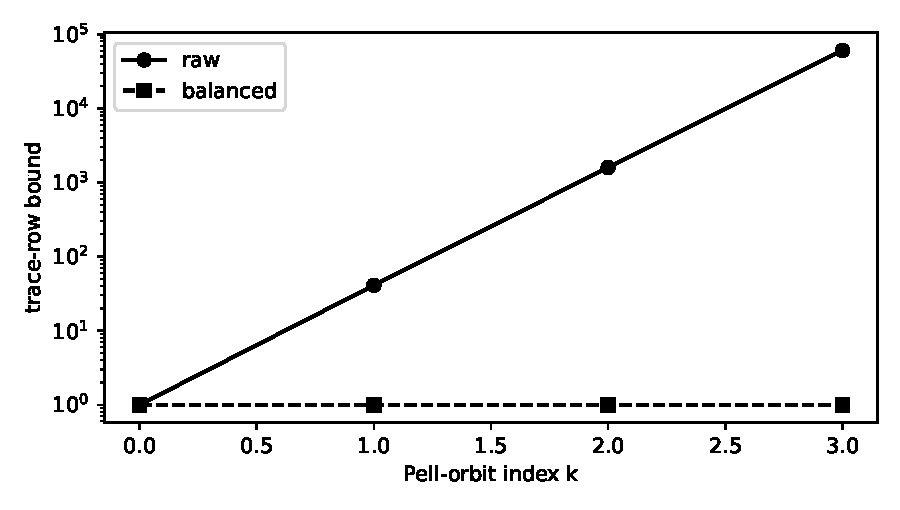
\includegraphics[width=0.72\textwidth]{sos_balancing_rows.pdf}
\Description{A log-scale line plot of the trace-row bound along a Pell orbit. The raw bound rises rapidly from k=0 to k=3, while the balanced bound remains constant.}
\caption{Raw and balanced trace-row bounds along the Pell orbit in the balancing ablation.}
\label{fig:sos-balance}
\end{figure}

\subsection*{Cross-field distributions and validation}

To probe the behaviour beyond $\OO_{10}$, Table~\ref{tab:crossfield} records exact-length
distributions for six representative fields and trace bound $80$. The last column
$\tau_{\max}$ denotes the smallest trace at which the maximal possible finite length $P(\OO_D)$
first appears.

\begin{table}[tbp]
\centering
\small
\renewcommand{\arraystretch}{1.12}
\begin{tabular}{rrrrrrrr}
\toprule
$D$ & $\#1$ & $\#2$ & $\#3$ & $\#4$ & $\#5$ & $\#\infty$ & $\tau_{\max}$ \\
\midrule
$5$ & $54$ & $576$ & $818$ & $0$ & $0$ & $0$ & $7$ \\
$10$ & $18$ & $87$ & $112$ & $29$ & $4$ & $270$ & $36$ \\
$13$ & $35$ & $256$ & $511$ & $78$ & $4$ & $14$ & $24$ \\
$29$ & $25$ & $130$ & $244$ & $121$ & $22$ & $60$ & $29$ \\
$53$ & $16$ & $75$ & $116$ & $85$ & $26$ & $126$ & $41$ \\
$101$ & $14$ & $32$ & $40$ & $28$ & $6$ & $200$ & $65$ \\
\bottomrule
\end{tabular}
\caption{Cross-field exact-length distributions for totally positive nonzero elements of trace at most $80$. The column $\tau_{\max}$ records the smallest trace at which the maximal length $P(\OO_D)$ first occurs.}
\label{tab:crossfield}
\end{table}

These data illustrate several phenomena already invisible in a single-field table. In the ternary
case $D=5$ every totally positive element of trace at most $80$ is representable and the maximal
length is already present at trace $7$. By contrast, for larger $D$ one sees substantial pools of
non-representable elements, together with a delayed first appearance of maximal-length elements.
Even among fields with $P(\OO_D)=5$, the distribution of lengths below trace $80$ changes
considerably with $D$.

Finally, we compared the package output against a separate brute-force coefficient-box validator.
It scans a naive coefficient box, does \emph{not} use the exact row-search engine, Peters'
criterion, or the closed-form Pythagoras classification, and reuses only the exact coefficient
arithmetic and embedding-comparison primitives from the ring layer.
The sweep covered every squarefree $D\le 41$ and every nonzero totally positive element of trace at most $24$.

\begin{table}[tbp]
\centering
\renewcommand{\arraystretch}{1.12}
\begin{tabular}{cccc}
\toprule
Fields checked & Trace bound & Elements compared & Mismatches \\
\midrule
$26$ & $24$ & $1358$ & $0$ \\
\bottomrule
\end{tabular}
\caption{Bounded-trace validation against a separate brute-force coefficient-box implementation.}
\label{tab:validation}
\end{table}

This validation sweep does not replace proof, but it provides a useful computational sanity check:
it confirms that the exact-length outputs agree with a deliberately naive coefficient-box search on
a substantial bounded corpus, without relying on Peters' criterion, the row-search engine, or the
closed-form Pythagoras classification. The sweep concerns lengths only; constructive decompositions
are checked separately in the bundled test suite.

\begin{remark}[Implementation]
The companion Python package \texttt{quadratic\_sos}, available at
\url{https://github.com/tomaszkania/quadratic_sos}, follows the exact-arithmetic philosophy of the
paper all the way through. The representability test already uses only exact coefficient
arithmetic by Proposition~\ref{prop:constant}. In the search phase, the implementation stores
points as coefficient pairs in the basis $1,\wD$ and computes each admissible row exactly: for a
fixed $v$, the trace inequality $\Tr(x^2)\le \Tr(\alpha)$ gives a finite enclosing interval for
$u$, and a directed binary search based on exact sign tests for $\sig_1$ and $\sig_2$ then locates
the precise interval of admissible integers on that row. No floating-point approximation is needed
for the search. The implementation also applies unit-square balancing before enumeration, using the
positive norm-one Pell unit discussed in Remark~\ref{rem:pell-balance}. It mirrors the paper's
mathematical assumptions at the API level: the constructor rejects non-squarefree radicands $D$,
and the exact-length and decomposition routines are defined only for nonzero inputs. The
repository contains a test suite reproducing the examples and Table~\ref{tab:data10}, together
with an executed notebook illustrating the algorithms. The scripts
\texttt{real\_quadratic\_sos\_table.py}, \texttt{balancing\_ablation.py},
\texttt{cross\_field\_distributions.py}, and \texttt{validation\_sweep.py}
compute the data underlying the computational study from this section. They are thin wrappers
importing the package routines, so the published computations and the library use the same
exact-arithmetic engine.
\end{remark}

\section*{Conclusion}

For maximal real quadratic orders, the exact length of a specific sum of integral squares can be
computed by a completely explicit finite algorithm. Peters' theorem decides representability,
corrected Minkowski bounds control the search geometry, exact trace-row enclosures and directed
bisection enumerate the relevant squares without floating-point arithmetic, and a
meet-in-the-middle argument distinguishes the exact lengths $1,2,3,4,5$.
The same framework also yields an explicit algorithm for the Pythagoras number and for an
integral Pythagoras element. The computational study shows in particular that the balancing step
is indispensable in practice: along Pell orbits it keeps the search geometry constant while the raw
trace-row bound grows explosively.

The present paper is intentionally conservative in its arithmetic input. A natural next step would
be to combine the finite-search approach with the continued-fraction theory of indecomposable
totally positive integers developed by Dress and Scharlau \cite{DressScharlau}, as in Ra\v ska's
work on the family-wise problem. Another direction is to import specialised low-rank criteria,
for instance Maa\ss's three-square criterion over $\OO_5$, into the exact-length algorithm as
field-specific short-circuits. Finally, it would be natural to extend the algorithm from maximal
real quadratic orders to arbitrary quadratic orders, where the exceptional order $\Z[\sqrt5]$
should already provide an instructive test case.

\section*{Conflict of interest}
The author declares that there is no conflict of interest.

\section*{Data availability}
No external data were gathered or used in this work. All computational tables and timings were
generated from the algorithms implemented in the companion repository at
\url{https://github.com/tomaszkania/quadratic_sos}; the submitted software component is version~0.2.0.

\bibliographystyle{ACM-Reference-Format}
\bibliography{references}


\end{document}
